\documentclass[a4paper,12pt]{article}

%%% Работа с русским языком
\usepackage{cmap}					% поиск в PDF
\usepackage{mathtext} 				% русские буквы в формулах
\usepackage[T2A]{fontenc}			% кодировка
\usepackage[utf8]{inputenc}			% кодировка исходного текста
\usepackage[english,russian]{babel}	% локализация и переносы
\usepackage{xcolor}
\usepackage{hyperref}
 % Цвета для гиперссылок
\definecolor{linkcolor}{HTML}{799B03} % цвет ссылок
\definecolor{urlcolor}{HTML}{799B03} % цвет гиперссылок

\hypersetup{pdfstartview=FitH,  linkcolor=linkcolor,urlcolor=urlcolor, colorlinks=true}

%%% Дополнительная работа с математикой
\usepackage{amsfonts,amssymb,amsthm,mathtools} % AMS
\usepackage{amsmath}
\usepackage{icomma} % "Умная" запятая: $0,2$ --- число, $0, 2$ --- перечисление

%% Номера формул
%\mathtoolsset{showonlyrefs=true} % Показывать номера только у тех формул, на которые есть \eqref{} в тексте.

%% Шрифты
\usepackage{euscript}	 % Шрифт Евклид
\usepackage{mathrsfs} % Красивый матшрифт

%% Свои команды
\DeclareMathOperator{\sgn}{\mathop{sgn}}

%% Перенос знаков в формулах (по Львовскому)
\newcommand*{\hm}[1]{#1\nobreak\discretionary{}
{\hbox{$\mathsurround=0pt #1$}}{}}
% графика
\usepackage{graphicx}
\graphicspath{{pictures/}}
\DeclareGraphicsExtensions{.pdf,.png,.jpg}
\author{Бурмашев Григорий, БПМИ-208}
\title{ТВиМС, дз -- 9}
\date{\today}
\begin{document}
\maketitle
\section*{Номер 8}
Знаем:
\[
\varrho_X(x) = Cx^{-4} ,  x \geq 1
\]
\[
\varrho_X(x) = 0, x < 1
\]
Из плотности сразу получаем (просто по определению):
\[
F_X(x) = \begin{cases}
\int\limits_1^x Cx^{-4}, x \geq 1 \\
0 , x < 1
\end{cases}
\]
\[
F_X(x) = \begin{cases}
1 - \frac{C}{3x^3}, x \geq 1 \\
0 , x < 1
\end{cases}
\]
Теперь ищем:
\subsection*{a)}
Мы знаем, что:
\[
\int_{-\infty}^{\infty} \varrho_X(x) dx = 1 
\]
\[
\int_{-\infty}^{1} \varrho_X(x) dx + \int_{1}^{\infty} \varrho_X(x) dx = 1 
\]
\[
0 + \int_{1}^{\infty} \varrho_X(x) dx = 1 
\]
Отсюда:
\[
\left(\frac{-C}{3x^3}\right) \Bigg|^a_1 \overset{a \rightarrow \infty }{=} 1
\]
\[
\frac{-C}{3a^3} + \frac{C}{3} = 1 \overset{a \rightarrow \infty }{=} \frac{C}{3}
\]
\[
\frac{C}{3} = 1
\]
\[
C = 3
\]

\subsection*{b)}
\[
Y = \frac{1}{X}, \varrho_Y(x) - ?
\]
\[
F_Y(x) = P(Y \leq x) = P(\frac{1}{X} \leq x) = \begin{cases}
P(X \geq \frac{1}{x}) , x > 0\\
0, x < 0 
\end{cases} = \begin{cases}
1 - P(X < \frac{1}{x}) , x > 0\\
0, x < 0 
\end{cases} = 
\]
\[
=
\begin{cases}
1 - P(X \leq \frac{1}{x}) , x > 0\\
0, x < 0 
\end{cases} \equiv
\begin{cases}
1 - P(X \leq 1) , x \geq 1 0\\
1 - P(X \leq \frac{1}{x}), x \in (0, 1)\\
0, x < 0
\end{cases} \equiv
\begin{cases}
1 , x \geq 1 \\
0 , x \leq 0  \\
1 - F_X(\frac{1}{x}), x \in (0, 1)
\end{cases}
\equiv 
\]
\[
\equiv
\begin{cases}
1 , x \geq 1 \\
0 , x \leq 0  \\ 
x^3, x \in (0, 1)
\end{cases}
\]
Отсюда получаем определение для плотности:
\[
\varrho_Y(x) = \begin{cases}
0, x \in (-\infty; 0] \cup [1, \infty) \\
(x^3)', x \in (0, 1)
\end{cases}
\]
\[
\varrho_Y(x) = \begin{cases}
0, x \in (-\infty; 0] \cup [1, \infty) \\
3x^2, x \in (0, 1)
\end{cases}
\]
\subsection*{c)}
\[
P(0.1 < Y < 0.3) - ?
\]
\[
P(0.1 < Y < 0.3)  = \int_{0.1}^{0.3} \varrho_Y(x) dx = \int_{0.1}^{0.3} 3x^2 dx = 3 \int_{0.1}^{0.3} x^2 dx
\]
\[
= 3 \cdot \frac{x^3}{3} \Bigg|^{0.3}_{0.1} = 3 \cdot \left(\frac{0.3^3 - 0.1^3}{3}\right) = \frac{13}{500}
\]
\begin{center}
\textbf{Ответ: } 
\[
C = 1
\]
\[
\varrho_Y(x) = \begin{cases}
0, x \in (-\infty; 0] \cup [1, \infty) \\
3x^2, x \in (0, 1)
\end{cases}
\]
\[
P(0.1 < Y < 0.3) = \frac{13}{500}
\]
\end{center}
\section*{Номер 9}
$X$ имеет равномерное распределение на $[0, 3]$, найти функцию распределения и плотность распределения:

Знаем:
\begin{center}

\includegraphics[scale=0.4]{1.png}
\end{center}
У нас отрезок $[0, 3]$, в таком случае мы хотим
\[
\varrho_X(x) = \begin{cases}
\frac{1}{3 - 0} , x \in [0, 3] \\
0, x \notin [0, 3]
\end{cases}
\]
Отсюда сразу получаем:
\[
F_X(x) = \begin{cases}
\frac{x}{3} , x \in [0, 3] \\
0, x \notin [0, 3]
\end{cases}
\]
Ну а теперь ищем:
\subsection*{a) $Y_1 = X^2$}
\[
F_{Y_1}(x) = P(Y_1 \leq x) = P(X^2 \leq x) = \begin{cases}
P(X \leq \sqrt{x}, x \geq 0) \\
0, x < 0
\end{cases} = \begin{cases}
F_X(\sqrt{x}), x \geq 0 \\
0, x < 0
\end{cases} = 
\]
\[
=
\begin{cases}
\frac{\sqrt{x}}{3}, \sqrt{x} \in [0, 3] \\
0, \sqrt{x} \notin [0, 3]
\end{cases}
\]
Ну а отсюда:
\[
\varrho_{Y_1}(x) = \begin{cases}
\frac{1}{6\sqrt{x}}, x \in [0, 9] \\
0, x \notin [0, 9]
\end{cases}
\]
\subsection*{b) $Y_2 = \sqrt{X}$}
Аналогично пункту \textbf{a)} получаем:
\[
P(Y_2 \leq x) = P(\sqrt{X} \leq x) = \begin{cases}
P(X \leq x^2), x \geq 0 \\
0 , x < 0
\end{cases}
=
\begin{cases}
F_X(x^2), x \geq 0 \\
0, x < 0 
\end{cases}
=
\begin{cases}
\frac{x^2}{3}, x^2 \in [0, 3] \\
0, x \notin [0, 3]
\end{cases}
\]
Отсюда:
\[
\varrho_{Y_2}(x) = \begin{cases}
\frac{2x}{3}, x \in [0, \sqrt{3}] \\
0, x \notin [0, \sqrt{3}]
\end{cases}
\]
\begin{center}
\textbf{Ответ: } 
\[
\varrho_{Y_1}(x) = \begin{cases}
\frac{1}{6\sqrt{x}}, x \in [0, 9] \\
0, x \notin [0, 9]
\end{cases}
\]
\[
\varrho_{Y_2}(x) = \begin{cases}
\frac{2x}{3}, x \in [0, \sqrt{3}] \\
0, x \notin [0, \sqrt{3}]
\end{cases}
\]
\end{center}
\clearpage
\section*{Номер 10}
\[
1 \leq |x| + |y| \leq 3, y > 0
\]
Найти функцию распределения и плотность случайной величины $X(x, y) = x$ и нарисовать график функции распределения
\\\\
Для начала посмотрим на график, нас интересует пересечение красного и зеленого участков:
\begin{center}

\includegraphics[scale=0.6]{2.png}
\end{center}
Разобьем наш график на промежутки и будем смотреть на них, заметим что площадь нашей фигуры равна 8, так что везде будем делить на $8$ для подсчета вероятности:
\begin{enumerate}
\item $x \in (-\infty, -3)$:

Вероятность равна нулю, очевидно
\item $x \in [-3, 1]$:
\[
\frac{1}{8} \cdot \left(\int_{-3}^x (t+3)dt \right) = \frac{1}{8} \left(\frac{t^2}{2} + 3t\right) \Bigg|^x_{-3} =  \frac{(x+3)^2}{16}
\]
\[
\varrho_x = \frac{x+3}{8}
\]
\item  $x \in [-1, 0]$:
\[
\frac18 \int_{-1}^{x} (t + 3) - (t+ 1)dt = \frac{1}{8} \int_{-1}^{x} 2dt = \frac{1}{8} \cdot (2t) \Bigg|^x_{-1} = \frac{2x+2}{8}
\]
\[
\varrho_x = \frac{1}{4}
\]
\item $x \in [0, 1]$:
\[ \frac{1}{8} \int_0^x ((3 - t) - (1 - t)) dt = \frac18 \int_0^x 2dt = \frac18 (2t) \Bigg|^x_0  = \frac{x}{4}
\]
\[
\varrho_x = \frac{1}{4}
\]
\item $x \in [1, 3]$:
\[
 \frac18 \int_1^x (3-t)dt = \frac18 (3t-\frac{t^2}{2})\Bigg|^x_1 = \frac18 \left(3x - \frac{x^2+5}{2}\right)
\]
\[
\varrho_x = \frac{3-x}{8}
\]
\item $x \in (3, \infty)$:

Вероятность равна единице, очевидно
\end{enumerate}
Терь считаем функцию распределения, когда будем переходить через каждую точку нужно прибавлять вероятность попадания в предыдущий промежуток. Всего у нас 4 промежутка, площади у них равны, а общая площадь 8, поэтому получаем:
\[
F(-1) = \text{как было} 
\]
\[
F(0) = \frac28 + \frac{2x+2}{8}  = \frac{2+x}{4}
\]
\[
F(1) = \frac{2}{8} + \frac28 +  \frac{x}{4}= \frac{2+x}{4}
\]
\[
F(3) = \frac28 + \frac28 + \frac28 + \frac18 \left(3x - \frac{x^2+5}{2}\right) = \frac{-x^2 + 6x + 7}{16}
\]
По итогу получаем:
\[
F_x(t) = 
\begin{cases}
0, t \in (-\infty, -3] \\
\frac{(t+3)^2}{16}, t \in (-3, -1] \\
\frac{2+t}{4}, t \in (-1, 1] \\
\frac{-x^2 + 6x + 7}{16}, t \in (1, 3) \\
1, t \in [3, \infty)
\end{cases}
\]
\[
\varrho_x(t) = 
\begin{cases}
0, t \in (-\infty, -3) \cup (3 , \infty) \\
\frac14, t \in [-1, 1] \\
\frac{t+3}{8}, t \in [-3, -1] \\
\frac{3-t}{8}, t \in [1, 3]
\end{cases}
\]
В таком случае график функции распределения:
\begin{center}
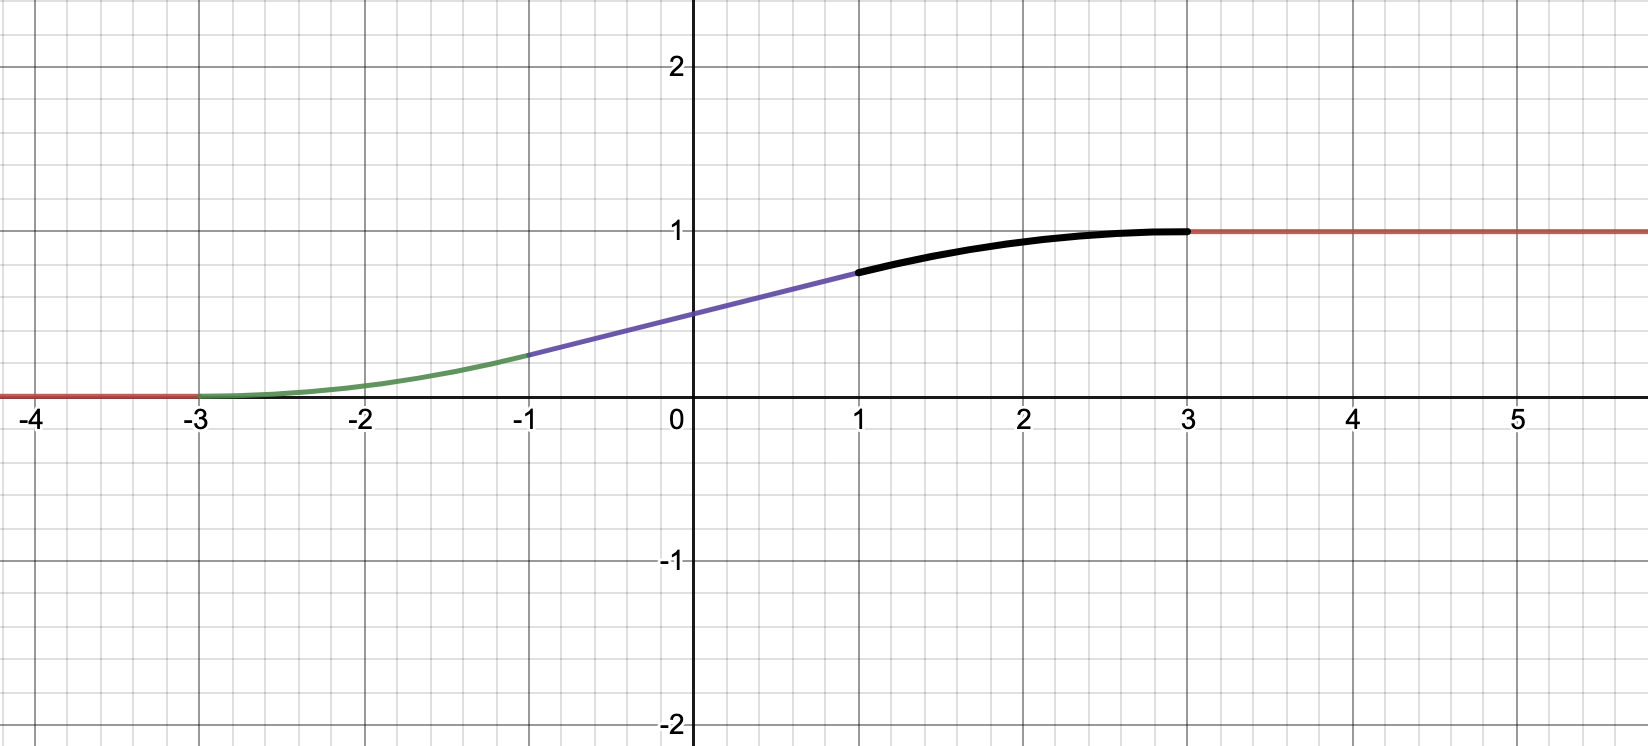
\includegraphics[scale=0.4]{3.png}
\end{center}
Где:
\begin{center}
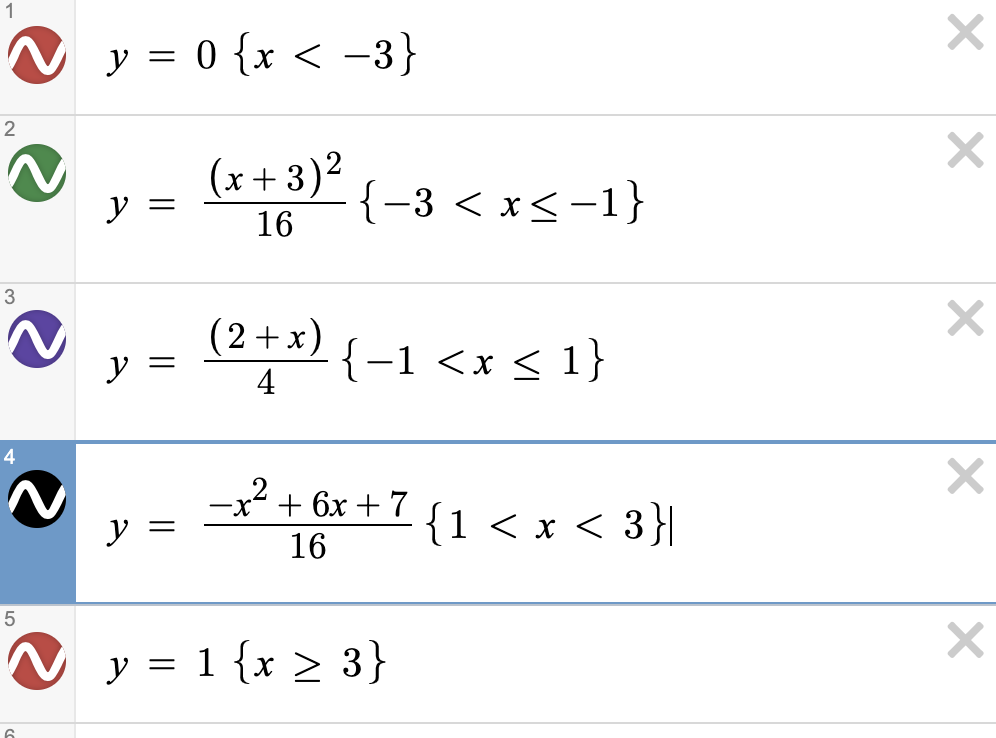
\includegraphics[scale=0.4]{4.png}
\end{center}
\end{document}
